% mnras_template.tex 
%
% LaTeX template for creating an MNRAS paper
%
% v3.0 released 14 May 2015
% (version numbers match those of mnras.cls)
%
% Copyright (C) Royal Astronomical Society 2015
% Authors:
% Keith T. Smith (Royal Astronomical Society)

% Change log
%
% v3.2 July 2023
%	Updated guidance on use of amssymb package
% v3.0 May 2015
%    Renamed to match the new package name
%    Version number matches mnras.cls
%    A few minor tweaks to wording
% v1.0 September 2013
%    Beta testing only - never publicly released
%    First version: a simple (ish) template for creating an MNRAS paper

%%%%%%%%%%%%%%%%%%%%%%%%%%%%%%%%%%%%%%%%%%%%%%%%%%
% Basic setup. Most papers should leave these options alone.
\documentclass[fleqn,usenatbib,openbib]{mnras}

% MNRAS is set in Times font. If you don't have this installed (most LaTeX
% installations will be fine) or prefer the old Computer Modern fonts, comment
% out the following line
\usepackage{newtxtext}
\usepackage[varvw]{newtxmath}
% Depending on your LaTeX fonts installation, you might get better results with one of these:
%\usepackage{mathptmx}
%\usepackage{txfonts}

% Use vector fonts, so it zooms properly in on-screen viewing software
% Don't change these lines unless you know what you are doing
\usepackage[T1]{fontenc}

% Allow "Thomas van Noord" and "Simon de Laguarde" and alike to be sorted by "N" and "L" etc. in the bibliography.
% Write the name in the bibliography as "\VAN{Noord}{Van}{van} Noord, Thomas"
\DeclareRobustCommand{\VAN}[3]{#2}
\let\VANthebibliography\thebibliography
\def\thebibliography{\DeclareRobustCommand{\VAN}[3]{##3}\VANthebibliography}


%%%%% AUTHORS - PLACE YOUR OWN PACKAGES HERE %%%%%

\usepackage[spanish]{babel}
\usepackage{lipsum}
\usepackage{url}
\usepackage{pgfplots}
\usepackage{booktabs, colortbl, bigstrut, multirow, multicol}

% Only include extra packages if you really need them. Avoid using amssymb if newtxmath is enabled, as these packages can cause conflicts. newtxmatch covers the same math symbols while producing a consistent Times New Roman font. Common packages are:
\usepackage{graphicx}	% Including figure files
\usepackage{amsmath}	% Advanced maths commands

%%%%%%%%%%%%%%%%%%%%%%%%%%%%%%%%%%%%%%%%%%%%%%%%%%

%%%%% AUTHORS - PLACE YOUR OWN COMMANDS HERE %%%%%

\usepackage[nameinlink,noabbrev]{cleveref}
\crefformat{figure}{\textsuperscript{#2#1#3}}
\crefformat{table}{\textsuperscript{#2#1#3}}

\addto\captionsspanish{\renewcommand{\refname}{REFERENCIAS}}

\makeatletter
\def\@abstract{\list{}{%
    \listparindent\realparindent
    \itemindent\z@
    \labelwidth\z@ \labelsep\z@
    \leftmargin\z@\rightmargin\z@%%was 11pc left
    \parsep 0pt plus 1pt}\item[]%
    \reset@font\normalsize{\bf PRESENTACIÓN}\\\reset@font\abslarge
} % SFB 0.1.01
\def\@keywords{\list{}{%
    \labelwidth\z@ \labelsep\z@
    \leftmargin\z@\rightmargin\z@  %was 11pc left was 11pc\right....
    \parsep 0pt plus 1pt}\item[]\reset@font\abslarge{\bf Palabras clave: }%
}
\makeatother

\renewcommand\theequation{\Alph{equation}}

% Please keep new commands to a minimum, and use \newcommand not \def to avoid
% overwriting existing commands. Example:
%\newcommand{\pcm}{\,cm$^{-2}$}	% per cm-squared

%%%%%%%%%%%%%%%%%%%%%%%%%%%%%%%%%%%%%%%%%%%%%%%%%%

%%%%%%%%%%%%%%%%%%% TITLE PAGE %%%%%%%%%%%%%%%%%%%

% Title of the paper, and the short title which is used in the headers.
% Keep the title short and informative.
\title[Velocidad del sonido]{Determinación de la velocidad del sonido y la constante adiabática del aire por medio de un tubo resonante}

% The list of authors, and the short list which is used in the headers.
% If you need two or more lines of authors, add an extra line using \newauthor
\author[Álvaro Jerónimo Sánchez]{
Álvaro Jerónimo Sánchez$^{1}$, DNI: 09847051S.\thanks{E-mail: alvaro.jeronimos@estudiante.uam.es}
Copartícipe: Hugo Pérez Hernández$^{1}$
\\
% List of institutions
$^{1}$Universidad Autónoma de Madrid, Ciudad universitaria de Cantoblanco, 28049,España \\
Facultad de Ciencias, Grado en Química, FÍSICA I
}

% These dates will be filled out by the publisher
\date{Prácticas 15/09/2023. Informe 22/10/2023. Fecha Límite 23/10/2023}

% Enter the current year, for the copyright statements etc.
\pubyear{2023}

% Don't change these lines
\begin{document}
\label{firstpage}
\pagerange{\pageref{firstpage}--\pageref{lastpage}}
\maketitle

%%%%%%%%%%%%%%%%%%%%%%%%%%%%%%%%%%%%%%%%%%%%%%%%%%

%%%%%%%%%%%%%%%%% BODY OF PAPER %%%%%%%%%%%%%%%%%%
\begin{abstract}

El sonido consiste en ondas longitudinales mecánicas resultantes de perturbaciones en el medio. Éste viajará a velocidades distintas según el medio en el que se encuentre y sus condiciones. Con esta práctica se pretende hallar su velocidad en el aire a temperatura ambiente, así como la constante adiabática del aire midiendo las longitudes a las que la onda se encuentra en resonancia a distintas frecuencias.

\vspace{1cm}
\end{abstract}

%%%%%%%%%%%%%%%%%%%%%%%%%%%%%%%%%%%%%%%%%%%%%%%%%%
\section{Teoría}

Cuando se genera una perturbación en un medio que hace vibrar al tímpano, dicha oscilación es convertida a impulso nervioso, que causa el estímulo del sonido \cite{bmc}. Las variaciones en la presión acústica son tan notables que se calculan con una escala logarítmica con la que se define la unidad de decibelios ($dB$). Las ondas sonoras son ondas mecánicas, ya que requieren un medio para propagarse, y longitudinales, ya que el desplazamiento es paralelo a la dirección de la onda. Las componentes de una onda son:

\begin{itemize}
    \item \textbf{Elongación ($x$):} Diferencia de la distancia de un punto al equilibrio.
    \item \textbf{Amplitud ($A$):} Elongación máxima de una onda en valor absoluto. 
    \item \textbf{Nodo:} Punto de una onda con mayor velocidad de oscilación ($v_o$).
    \item \textbf{Vientre:} Espacio entre nodo y nodo.
    \item \textbf{Longitud de onda ($\lambda$):} Distancia entre dos nodos de una onda.
    \item \textbf{Frecuencia ($\nu$):} Número de oscilaciones que ocurren en un tiempo determinado. Su inversa es el \textbf{periodo}.
    \item \textbf{Fase($\phi$):} Define el estado oscilatorio de la onda. Ángulo que hay entre el equilibrio y un punto de una onda en un instante (en radianes).
\end{itemize}

En este caso se trata de una onda en un sistema cerrado, ya que para la práctica se ha dispuesto un altavoz de frecuencia modulable contenido en un tubo de longitud ($L$) variable (aunque, al haber un pequeño orificio por la parte inferior del tubo, parte de la onda se propaga fuera del sistema, hecho que se ha tenido en cuenta posteriormente en los cálculos). Esto causará que las ondas reboten e interfieran unas con otras, en la mayoría de los casos contrarrestándose (causando una interferencia destructiva) y haciendo que el volumen disminuya considerablemente. Con ciertas combinaciones de frecuencia ($\nu$) y longitud ($L$), se puede conseguir una resonancia, es decir, que las ondas que ''rebotan'' oscilen en conjunto, sumándose las intensidades, causando una interferencia constructiva \cite{hund} y haciendo que el volumen aumente. En esta práctica se ha aprovechado dicho fenómeno para determinar a qué longitudes se produce la resonancia dentro de varias frecuencias fijas, datos que posteriormente se han usado para calcular la velocidad del sonido. Ésta fluctuará dependiendo del medio por el que se propaga el sonido y la temperatura a la que éste se encuentra, variando así según el coeficiente adiabático del medio ($\gamma$), dato que también se ha determinado en los cálculos.

\begin{figure}
    \centering
    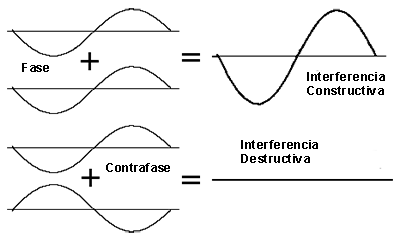
\includegraphics[width=\columnwidth]{interferencia.png}
    \caption{Interferencia constructiva y destructiva \protect\cite{img}}
    \label{fig:interferencia}
    \end{figure}

%%%%%%%%%%%%%%%%%%%%%%%%%%%%%%%%%%%%%%%%%%%%%%%%%%
\section{Montaje experimental}

\subsection{Instrumentos}

El aparato usado en esta práctica consistía en un tubo de Pyrex (de $~23$ mm de diámetro interior) unido a una base metálica con un altavoz woofer. En la parte superior del tubo había un émbolo con el que variar la longitud del mismo y, adyacente a éste, había anclada una regla milimetrada para poder medir dicha longitud. Para ajustar la frecuencia emitida, el altavoz estaba conectado a un oscilador electrónico que también permitía aumentar o disminuir la amplitud de onda, incrementando o disminuyendo así el volumen general.

% Table generated by Excel2LaTeX from sheet 'Sheet3'
\begin{table*}
  \centering
  \caption{Longitudes $L$ (y $\Delta L_{Ef}$) en las que existía resonancia para cada frecuencia}
    \begin{tabular}{|c|ccc|c|cc|c|cc|c|c|}
\cline{1-11}    \rowcolor[rgb]{ .788,  .788,  .788} \multicolumn{2}{|c|}{} & \multicolumn{9}{c|}{Frecuencia ($\nu$)}                               & \multicolumn{1}{c}{\cellcolor[rgb]{ 1,  1,  1}} \bigstrut\\
\cline{2-11}    \rowcolor[rgb]{ .788,  .788,  .788}       & \multicolumn{1}{c|}{\cellcolor[rgb]{ .949,  .949,  .949}\textcolor[rgb]{ .247,  .247,  .247}{\textbf{Orden}}} & \multicolumn{3}{c|}{\cellcolor[rgb]{ .949,  .949,  .949}\textcolor[rgb]{ .247,  .247,  .247}{\textbf{2000  Hz}}} & \multicolumn{3}{c|}{\cellcolor[rgb]{ .949,  .949,  .949}\textcolor[rgb]{ .247,  .247,  .247}{\textbf{1500  Hz}}} & \multicolumn{3}{c|}{\cellcolor[rgb]{ .949,  .949,  .949}\textcolor[rgb]{ .247,  .247,  .247}{\textbf{1000 Hz}}} & \multicolumn{1}{c}{\cellcolor[rgb]{ 1,  1,  1}} \bigstrut\\
\cline{2-11}    \rowcolor[rgb]{ .788,  .788,  .788}       & \multicolumn{1}{c|}{\cellcolor[rgb]{ .929,  .929,  .929}k} & \multicolumn{1}{c|}{\cellcolor[rgb]{ .929,  .929,  .929}$L$ (m)} & \cellcolor[rgb]{ .929,  .929,  .929}$L_{Ef}$ (m) & \cellcolor[rgb]{ .929,  .929,  .929}$v$ (m/s) & \multicolumn{1}{c|}{\cellcolor[rgb]{ .929,  .929,  .929}$L$ (m)} & \cellcolor[rgb]{ .929,  .929,  .929}$L_{Ef}$ (m) & \cellcolor[rgb]{ .929,  .929,  .929}$v$ (m/s) & \multicolumn{1}{c|}{\cellcolor[rgb]{ .929,  .929,  .929}$L$ (m)} & \cellcolor[rgb]{ .929,  .929,  .929}$L_{Ef}$ (m) & \cellcolor[rgb]{ .929,  .929,  .929}$v$ (m/s) & \multicolumn{1}{c}{\cellcolor[rgb]{ 1,  1,  1}} \bigstrut\\
\cline{2-11}    \rowcolor[rgb]{ .788,  .788,  .788}       & \multicolumn{1}{c|}{\cellcolor[rgb]{ 1,  1,  1}0} & \multicolumn{1}{c|}{\cellcolor[rgb]{ 1,  1,  1}0.037} & \cellcolor[rgb]{ 1,  1,  1}0.044 & \cellcolor[rgb]{ 1,  1,  1}351.200 & \multicolumn{1}{c|}{\cellcolor[rgb]{ 1,  1,  1}0.051} & \cellcolor[rgb]{ 1,  1,  1}0.058 & \cellcolor[rgb]{ 1,  1,  1}347.400 & \multicolumn{1}{c|}{\cellcolor[rgb]{ 1,  1,  1}0.084} & \cellcolor[rgb]{ 1,  1,  1}0.091 & \cellcolor[rgb]{ 1,  1,  1}363.600 & \multicolumn{1}{c}{\cellcolor[rgb]{ 1,  1,  1}} \bigstrut\\
\cline{2-11}    \rowcolor[rgb]{ .788,  .788,  .788}       & \multicolumn{1}{c|}{\cellcolor[rgb]{ 1,  1,  1}1} & \multicolumn{1}{c|}{\cellcolor[rgb]{ 1,  1,  1}0.129} & \cellcolor[rgb]{ 1,  1,  1}0.136 & \cellcolor[rgb]{ 1,  1,  1}362.400 & \multicolumn{1}{c|}{\cellcolor[rgb]{ 1,  1,  1}0.164} & \cellcolor[rgb]{ 1,  1,  1}0.171 & \cellcolor[rgb]{ 1,  1,  1}341.800 & \multicolumn{1}{c|}{\cellcolor[rgb]{ 1,  1,  1}0.256} & \cellcolor[rgb]{ 1,  1,  1}0.263 & \cellcolor[rgb]{ 1,  1,  1}350.533 & \multicolumn{1}{c}{\cellcolor[rgb]{ 1,  1,  1}} \bigstrut\\
\cline{2-11}    \rowcolor[rgb]{ .788,  .788,  .788}       & \multicolumn{1}{c|}{\cellcolor[rgb]{ 1,  1,  1}2} & \multicolumn{1}{c|}{\cellcolor[rgb]{ 1,  1,  1}0.218} & \cellcolor[rgb]{ 1,  1,  1}0.225 & \cellcolor[rgb]{ 1,  1,  1}359.840 & \multicolumn{1}{c|}{\cellcolor[rgb]{ 1,  1,  1}0.281} & \cellcolor[rgb]{ 1,  1,  1}0.288 & \cellcolor[rgb]{ 1,  1,  1}345.480 & \multicolumn{1}{c|}{\cellcolor[rgb]{ 1,  1,  1}0.430} & \cellcolor[rgb]{ 1,  1,  1}0.437 & \cellcolor[rgb]{ 1,  1,  1}349.520 & \multicolumn{1}{c}{\cellcolor[rgb]{ 1,  1,  1}} \bigstrut\\
\cline{2-11}    \rowcolor[rgb]{ .788,  .788,  .788}       & \multicolumn{1}{c|}{\cellcolor[rgb]{ 1,  1,  1}3} & \multicolumn{1}{c|}{\cellcolor[rgb]{ 1,  1,  1}0.307} & \cellcolor[rgb]{ 1,  1,  1}0.314 & \cellcolor[rgb]{ 1,  1,  1}358.743 & \multicolumn{1}{c|}{\cellcolor[rgb]{ 1,  1,  1}0.397} & \cellcolor[rgb]{ 1,  1,  1}0.404 & \cellcolor[rgb]{ 1,  1,  1}346.200 & \multicolumn{1}{c|}{\cellcolor[rgb]{ 1,  1,  1}0.605} & \cellcolor[rgb]{ 1,  1,  1}0.612 & \cellcolor[rgb]{ 1,  1,  1}349.657 & \multicolumn{1}{c}{\cellcolor[rgb]{ 1,  1,  1}} \bigstrut\\
\cline{2-11}    \rowcolor[rgb]{ .788,  .788,  .788}       & \multicolumn{1}{c|}{\cellcolor[rgb]{ 1,  1,  1}4} & \multicolumn{1}{c|}{\cellcolor[rgb]{ 1,  1,  1}0.400} & \cellcolor[rgb]{ 1,  1,  1}0.407 & \cellcolor[rgb]{ 1,  1,  1}361.689 & \multicolumn{1}{c|}{\cellcolor[rgb]{ 1,  1,  1}0.503} & \cellcolor[rgb]{ 1,  1,  1}0.510 & \cellcolor[rgb]{ 1,  1,  1}339.933 & \multicolumn{1}{c|}{\cellcolor[rgb]{ 1,  1,  1}0.749} & \cellcolor[rgb]{ 1,  1,  1}0.756 & \cellcolor[rgb]{ 1,  1,  1}335.956 & \multicolumn{1}{c}{\cellcolor[rgb]{ 1,  1,  1}} \bigstrut\\
\cline{2-11}    \rowcolor[rgb]{ .788,  .788,  .788}       & \multicolumn{1}{c|}{\cellcolor[rgb]{ 1,  1,  1}5} & \multicolumn{1}{c|}{\cellcolor[rgb]{ 1,  1,  1}0.488} & \cellcolor[rgb]{ 1,  1,  1}0.495 & \cellcolor[rgb]{ 1,  1,  1}359.927 & \multicolumn{1}{c|}{\cellcolor[rgb]{ 1,  1,  1}0.635} & \cellcolor[rgb]{ 1,  1,  1}0.642 & \cellcolor[rgb]{ 1,  1,  1}350.127 & \multicolumn{1}{c|}{\cellcolor[rgb]{ 1,  1,  1}0.900} & \cellcolor[rgb]{ 1,  1,  1}0.907 & \cellcolor[rgb]{ 1,  1,  1}329.782 & \multicolumn{1}{c}{\cellcolor[rgb]{ 1,  1,  1}} \bigstrut\\
\cline{2-10}    \rowcolor[rgb]{ .788,  .788,  .788}       & \multicolumn{1}{c|}{\cellcolor[rgb]{ 1,  1,  1}6} & \multicolumn{1}{c|}{\cellcolor[rgb]{ 1,  1,  1}0.572} & \cellcolor[rgb]{ 1,  1,  1}0.579 & \cellcolor[rgb]{ 1,  1,  1}356.246 & \multicolumn{1}{c|}{\cellcolor[rgb]{ 1,  1,  1}0.762} & \cellcolor[rgb]{ 1,  1,  1}0.769 & \cellcolor[rgb]{ 1,  1,  1}354.877 & \multicolumn{2}{c|}{\multirow{6}[11]{*}{\cellcolor[rgb]{ 0,  0,  0}}} & \multicolumn{1}{c}{\multirow{6}[11]{*}{\cellcolor[rgb]{ 0,  0,  0}}} & \multicolumn{1}{c}{\cellcolor[rgb]{ 1,  1,  1}} \bigstrut\\
\cline{2-8}    \rowcolor[rgb]{ .788,  .788,  .788}       & \multicolumn{1}{c|}{\cellcolor[rgb]{ 1,  1,  1}7} & \multicolumn{1}{c|}{\cellcolor[rgb]{ 1,  1,  1}0.657} & \cellcolor[rgb]{ 1,  1,  1}0.664 & \cellcolor[rgb]{ 1,  1,  1}354.080 & \multicolumn{1}{c|}{\cellcolor[rgb]{ 1,  1,  1}0.848} & \cellcolor[rgb]{ 1,  1,  1}0.855 & \cellcolor[rgb]{ 1,  1,  1}341.960 & \multicolumn{2}{c|}{\cellcolor[rgb]{ 0,  0,  0}} & \multicolumn{1}{c}{\cellcolor[rgb]{ 0,  0,  0}} & \multicolumn{1}{c}{\cellcolor[rgb]{ 1,  1,  1}} \bigstrut\\
\cline{2-7}    \rowcolor[rgb]{ .788,  .788,  .788}       & \multicolumn{1}{c|}{\cellcolor[rgb]{ 1,  1,  1}8} & \multicolumn{1}{c|}{\cellcolor[rgb]{ 1,  1,  1}0.705} & \cellcolor[rgb]{ 1,  1,  1}0.712 & \cellcolor[rgb]{ 1,  1,  1}335.012 & \multicolumn{2}{r|}{\multirow{4}[7]{*}{\cellcolor[rgb]{ 0,  0,  0}}} & \multirow{4}[7]{*}{\cellcolor[rgb]{ 0,  0,  0}} & \multicolumn{2}{c|}{\cellcolor[rgb]{ 0,  0,  0}} & \multicolumn{1}{c}{\cellcolor[rgb]{ 0,  0,  0}} & \multicolumn{1}{c}{\cellcolor[rgb]{ 1,  1,  1}} \bigstrut\\
\cline{2-5}    \rowcolor[rgb]{ .788,  .788,  .788}       & \multicolumn{1}{c|}{\cellcolor[rgb]{ 1,  1,  1}9} & \multicolumn{1}{c|}{\cellcolor[rgb]{ 1,  1,  1}0.750} & \cellcolor[rgb]{ 1,  1,  1}0.757 & \cellcolor[rgb]{ 1,  1,  1}318.695 & \multicolumn{2}{r|}{\cellcolor[rgb]{ 0,  0,  0}} & \cellcolor[rgb]{ 0,  0,  0} & \multicolumn{2}{c|}{\cellcolor[rgb]{ 0,  0,  0}} & \multicolumn{1}{c}{\cellcolor[rgb]{ 0,  0,  0}} & \multicolumn{1}{c}{\cellcolor[rgb]{ 1,  1,  1}} \bigstrut\\
\cline{2-5}    \rowcolor[rgb]{ .788,  .788,  .788}       & \multicolumn{1}{c|}{\cellcolor[rgb]{ 1,  1,  1}10} & \multicolumn{1}{c|}{\cellcolor[rgb]{ 1,  1,  1}0.832} & \cellcolor[rgb]{ 1,  1,  1}0.839 & \cellcolor[rgb]{ 1,  1,  1}319.581 & \multicolumn{2}{r|}{\cellcolor[rgb]{ 0,  0,  0}} & \cellcolor[rgb]{ 0,  0,  0} & \multicolumn{2}{c|}{\cellcolor[rgb]{ 0,  0,  0}} & \multicolumn{1}{c}{\cellcolor[rgb]{ 0,  0,  0}} & \multicolumn{1}{c}{\cellcolor[rgb]{ 1,  1,  1}} \bigstrut\\
\cline{2-5}    \rowcolor[rgb]{ .788,  .788,  .788}       & \multicolumn{1}{c|}{\cellcolor[rgb]{ 1,  1,  1}11} & \multicolumn{1}{c|}{\cellcolor[rgb]{ 1,  1,  1}0.900} & \cellcolor[rgb]{ 1,  1,  1}0.907 & \cellcolor[rgb]{ 1,  1,  1}315.443 & \multicolumn{2}{r|}{\cellcolor[rgb]{ 0,  0,  0}} & \cellcolor[rgb]{ 0,  0,  0} & \multicolumn{2}{c|}{\cellcolor[rgb]{ 0,  0,  0}} & \multicolumn{1}{c}{\cellcolor[rgb]{ 0,  0,  0}} & \multicolumn{1}{c}{\cellcolor[rgb]{ 1,  1,  1}} \bigstrut[t]\\
    \rowcolor[rgb]{ .788,  .788,  .788} Promedio & \cellcolor[rgb]{ 1,  1,  1} & \cellcolor[rgb]{ 1,  1,  1} & \cellcolor[rgb]{ 1,  1,  1} & \cellcolor[rgb]{ .949,  .949,  .949}\textcolor[rgb]{ .247,  .247,  .247}{\textbf{346.071}} & \cellcolor[rgb]{ 1,  1,  1} & \cellcolor[rgb]{ 1,  1,  1} & \cellcolor[rgb]{ .949,  .949,  .949}\textcolor[rgb]{ .247,  .247,  .247}{\textbf{345.972}} & \cellcolor[rgb]{ 1,  1,  1} & \cellcolor[rgb]{ 1,  1,  1} & \cellcolor[rgb]{ .949,  .949,  .949}\textcolor[rgb]{ .247,  .247,  .247}{\textbf{346.508}} & \cellcolor[rgb]{ .949,  .949,  .949}\textcolor[rgb]{ .98,  .49,  0}{\textbf{346.184}} \\
    \end{tabular}%
  \label{tab:tab1}%
\end{table*}%

\subsection{Medición}

Con la longitud del tubo al máximo (el émbolo subido lo más alto posible), se fijó la frecuencia en $2000$ Hz y se comenzó a bajar el émbolo lentamente, tratando de escuchar los máximos y mínimos de volumen (correspondiendo a los vientres y nodos de la onda, respectivamente) y anotando los valores de la longitud para los que el volumen era mayor. Para escuchar la diferencia lo mejor posible, se configuró la amplitud al máximo. Una vez extenuada la longitud del tubo, se repitió el procedimiento cambiando la frecuencia a $1500$ Hz y $1000$ Hz. Como era de esperar, para las frecuencias más altas la onda tuvo oscilaciones más cortas, lo que causó un mayor registro de máximos (mayor número de longitudes del tubo en las que existía resonancia), como se ve reflejado en la tabla \cref{tab:tab1}.

\vspace{2cm}
\begin{figure}
\centering
\caption{Gráfica Longitud-Número de ondas para cada frecuencia}
\label{fig:graph}
\begin{tikzpicture}[scale=0.8]
\begin{axis}[legend entries={2000 Hz, 1500 Hz, 1000 Hz},
legend style={
at={(0.5,-0.2)},
anchor=north,
legend columns=1,
cells={anchor=west},
font=\footnotesize,
rounded corners=2pt,
}, 
reverse legend, legend pos=outer north east,xlabel=k (número de ondas), ylabel=$L$ (m),
axis lines=middle,grid=major,grid style={dashed}
]
\addplot table [x=k, y=2000 Hz,, col sep=comma] {mydata.csv};
\addplot table [x=k, y=1500 Hz, col sep=comma] {mydata.csv};
\addplot table [x=k, y=1000 Hz, col sep=comma] {mydata.csv};
\end{axis}
\end{tikzpicture}
\end{figure}

%%%%%%%%%%%%%%%%%%%%%%%%%%%%%%%%%%%%%%%%%%%%%%%%%%
\section{Cálculos}

Debido a que en el extremo abierto del tubo las ondas se propagan hacia todas las direcciones, es necesario calcular una longitud efectiva ($L_{Ef}$), que será la que utilizaremos para los cálculos \cite{labuam}. La diferencia entre ésta y la longitud ($L$) real será menor cuanto mayor sea $L$ respecto al radio ($r$) del tubo. Se ha calculado $L_{Ef}$ con su expresión, resultados que vienen reflejados en la tabla\cref{tab:tab1}:

\begin{gather}
    L_{Ef} = L+0.6r
\end{gather}

Para que se dé la resonancia debe haber un nodo en el émbolo y se debe formar un vientre en la boca del tubo. Para que se cumplan estas condiciones, los vientres intermedios deben dividir al tubo en un número impar de partes de longitud $\lambda/4$, siendo $v/\nu$ la longitud de onda \cite{labuam}, por lo que $L$ vendrá dada por:

\begin{gather}
    L = (2K+1)\frac{\lambda}{4} = (2K+1)\frac{v}{4\nu}
\end{gather}

Despejando la velocidad ($v$) de dicha expresión [B] y sustituyendo la longitud ($L$) por $L_{Ef}$ obtenemos la siguiente expresión:

\begin{gather}
    v = \frac{4L_{Ef}\nu}{2K+1}
\end{gather}

Con esta expresión [C] se han calculado todos los valores de la velocidad del sonido para cada set de datos, como está reflejado en la tabla\cref{tab:tab1}. Haciendo el promedio de los datos con las distintas frecuencias, el resultado de la velocidad del sonido a $25$ °C en el aire ha sido de: \boxed{$346.2$ m/s}. \bigskip


Debido a que las variaciones de presión que produce la onda en el aire son relativamente rápidas \cite{labuam}, se ha podido considerar que no hay intercambio de calor con el exterior (es un proceso adiabático), por lo que la velocidad del sonido en el aire viene dada por:

\begin{gather}
    v = \sqrt{\gamma\frac{RT}{M}}
\end{gather}

Siendo $R$ la constante de los gases ideales ($8.314\; J/mol\cdot K$), y $M$ la masa molar del aire ($29.96\pm0.01\; g/mol$).

Para calcular el coeficiente adiabático del medio, en este caso del aire, ha habido que tener en cuenta la temperatura actual. En el día de la prueba había una temperatura de $25$ °C ($298.15$ K), como se ha mencionado anteriormente. Despejando $\gamma$ de la ecuación [D] y usando los datos mencionados anteriormente, así como el promedio hallado de la velocidad del sonido, se ha obtenido el siguiente valor del coeficiente adiabático del aire:

\begin{gather}
    \gamma = \frac{v^{2}M}{RT} = \boxed{1.448}
\end{gather}

\subsection{Errores}

El error del oscilador entre las líneas que indicaban valores de frecuencia era grande, de $\pm5$ Hz pero, al ser los valores de frecuencia trabajados coincidentes con los valores marcados en el contador, se sabía con certeza hasta la primera cifra decimal, reduciéndose el error a $\pm0.5$ Hz. Al derivar la fórmula [C] por cada una de sus variables (k tiene precisión infinita, por lo que no hay error que propague) y redistribuirla en sumas, podemos hallar el error sistemático del cálculo de la velocidad:

\begin{align}
    & \frac{\Delta v}{v} = \frac{\Delta L_{Ef}}{L_{Ef}}+\frac{\Delta\nu}{\nu}\\
    & \Delta v = v(\frac{\Delta L_{Ef}}{L_{Ef}}+\frac{\Delta\nu}{\nu})
\end{align}

Sustituyendo datos, teniendo en cuenta que el error del oscilador es de $\pm0.5$ Hz y el de la regla milimetrada $\pm0.5\cdot10^{-3}$ m, obtenemos que el error del resultado promedio de la velocidad del sonido es:

\begin{gather}
    \Delta v = 346.2(\frac{0.0005}{0.044}+\frac{0.5}{1000}) = \boxed{4.1}
\end{gather}
\textit{(NOTA: se han usado los valores de $\nu$ y $L_{Ef}$ más pequeños en la fórmula, ya que supondrá un mayor error total, y los errores se calculan de manera pesimista)}

Repitiendo el proceso para el coeficiente adiabático ($\gamma$), teniendo en cuenta que el error de $M$ es $\pm0.01$, el de $v$ $\pm4.1$ y el de $T$ $\pm0.005$ (en las mismas unidades que los datos usados para los cálculos), hallamos que su error es:

\begin{gather}
    \Delta\gamma = \gamma(2\frac{\Delta v}{v}+\frac{\Delta M}{M}+\frac{\Delta T}{T}) = \boxed{0.035}
\end{gather}

\smallskip

La desviación típica es el valor al que tienden a desviarse los cálculos propios a partir de las medidas tomadas. En vez de tener en cuenta errores sistemáticos, está relacionado con errores aleatorios. Aplicando la definición, se ha obtenido que la desviación típica de la velocidad del sonido es:

\begin{gather}
    \sigma = \sqrt{\frac{\sum\limits_{i=1}^{n}(v-v_{media})^2}{n-1}} = \boxed{13.63}
\end{gather}

\pagebreak
\subsection{Resultados}

Comparando los resultados obtenidos con medidas de otros estudios (realizados de manera más profesional), a pesar del error que lo acompaña, el valor para la velocidad del sonido en el aire a $20$ °C parece ser prácticamente exacto. Igualmente, la cifra del coeficiente adiabático es notablemente próxima a lo esperado.

% Table generated by Excel2LaTeX from sheet 'Sheet4'
\begin{table}
  \centering
  \caption{Resultados}
    \begin{tabular}{|l|r|l|r|}
    \hline
    \rowcolor[rgb]{ .788,  .788,  .788} \multicolumn{4}{|c|}{\textsc{Resultados}} \bigstrut\\
    \hline
    \rowcolor[rgb]{ .929,  .929,  .929}       & \multicolumn{1}{l|}{Valor} & $\Delta x$ & \multicolumn{1}{l|}{$\sigma$} \bigstrut\\
    \hline
    \rowcolor[rgb]{ .929,  .929,  .929} $v$   & \cellcolor[rgb]{ 1,  1,  1}346.2 & \cellcolor[rgb]{ 1,  1,  1}$\pm4.1$ & \multicolumn{1}{l|}{\cellcolor[rgb]{ 1,  1,  1}$\pm13.63$} \bigstrut\\
    \hline
    \rowcolor[rgb]{ .929,  .929,  .929} $\gamma$ & \cellcolor[rgb]{ 1,  1,  1}1.448 & \cellcolor[rgb]{ 1,  1,  1}$\pm0.035$ & \cellcolor[rgb]{ 0,  0,  0} \bigstrut\\
    \hline
    \end{tabular}%
  \label{tab:results}%
\end{table}%

%%%%%%%%%%%%%%%%%%%%%%%%%%%%%%%%%%%%%%%%%%%%%%%%%%
\section{Complicaciones}

Al ser la segunda práctica de laboratorio y haber leído el guión rigurosamente antes de comenzar el proceso de medición, no ha habido muchas complicaciones en el experimento. No obstante, incluso al volumen máximo, mi copartícipe, asignado en un principio a escuchar los máximos de la onda, tuvo dificultades para discernir el sonido del altavoz (cabe mencionar que otro grupo estaba realizando la misma práctica simultáneamente, dificultando la escucha debido a la contaminación acústica) y fue necesario cambiar cargos. 

%%%%%%%%%%%%%%%%%%%%%%%%%%%%%%%%%%%%%%%%%%%%%%%%%%
\section{Conclusión}

Tras realizar todos los cálculos y observar los resultados, se han obtenido valores sumamente cercanos a los registrados por estudios de mayor escala, y se ha podido observar cómo la teoría presentada en el guión \cite{labuam} se cumple. Se ha observado cómo el número de ondas reducía al bajar la frecuencia, y cómo dicho número se ha mantenido impar para todos los casos. Tomando en consideración todo lo expuesto, se ha concluido el experimento de manera satisfactoria.

%%%%%%%%%%%%%%%%%%%% REFERENCES %%%%%%%%%%%%%%%%%%

% The best way to enter references is to use BibTeX:

\nocite{*}
\bibliographystyle{mnras}
\bibliography{bibliography}


% Alternatively you could enter them by hand, like this:
% This method is tedious and prone to error if you have lots of references
%\begin{thebibliography}{99}
%\bibitem[\protect\citeauthoryear{Author}{2012}]{Author2012}
%Author A.~N., 2013, Journal of Improbable Astronomy, 1, 1
%\bibitem[\protect\citeauthoryear{Others}{2013}]{Others2013}
%Others S., 2012, Journal of Interesting Stuff, 17, 198
%\end{thebibliography}

%%%%%%%%%%%%%%%%%%%%%%%%%%%%%%%%%%%%%%%%%%%%%%%%%%

%%%%%%%%%%%%%%%%% APPENDICES %%%%%%%%%%%%%%%%%%%%%

\pagebreak

\begin{figure}
    \centering
    \includegraphics[width=\textwidth]{sonido.png}
    \end{figure}

%%%%%%%%%%%%%%%%%%%%%%%%%%%%%%%%%%%%%%%%%%%%%%%%%%


% Don't change these lines
\bsp	% typesetting comment
\label{lastpage}
\end{document}

% End of mnras_template.tex